\documentclass{beamer}
\usepackage{color,amsmath,comment, subfigure}
\usepackage{booktabs}
\def\vf{\vfill}
\usepackage{url}

%%%%%%%%%%%%%%%%%%%%%%%%%%
\title[]{Introduction}
\author[]{Matthew J. Salganik}
\institute[]{Social Network (Soc 204)\\Spring 2017\\Princeton University}
\date[]{February 6, 2017

\vf 

\begin{flushright}
\vspace{0.6in}

\includegraphics[width=0.1\textwidth]{figures/cc.png}
\end{flushright}

}

\begin{document}
%%%%%%%%%%%%%%%%%%%%%%%%%%%
\frame{\titlepage}
%%%%%%%%%%%%%%%%%%%%%%%%%%%
\begin{frame}


\begin{center}

\includegraphics[height=0.50\textheight]{figures/watts_six_2003_cover}
\end{center}

\vf

\begin{center}
\Large{
We live in the connected age.
}
\end{center}

\end{frame}
%%%%%%%%%%%%%%%%%%%%%%%%%%%
\begin{frame}

\begin{center}
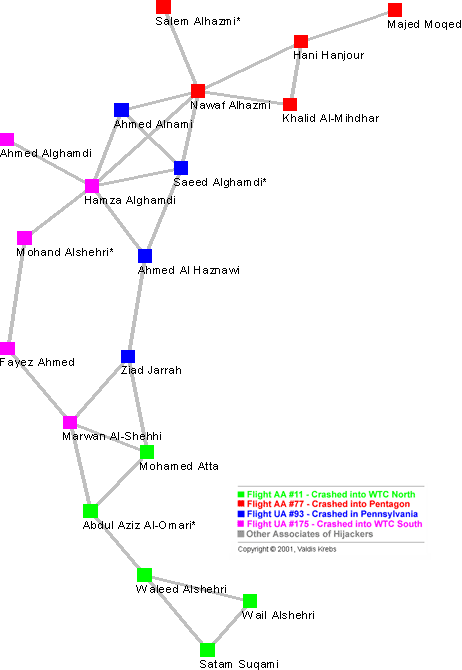
\includegraphics[height=0.90\textheight]{figures/krebs_uncloaking_2002_fig2}
\end{center}

\vf
\Tiny{\url{http://pear.accc.uic.edu/ojs/index.php/fm/article/view/941/863}}

\end{frame}
%%%%%%%%%%%%%%%%%%%%%%%%%%%
\begin{frame}

\begin{center}
\includegraphics<1>[width=0.95\textwidth]{figures/madoff}
\end{center}

\vf
\Tiny{\url{http://www.orgnet.com/madoff.html}}

\end{frame}
%%%%%%%%%%%%%%%%%%%%%%%%%%%
\begin{frame}

\begin{center}
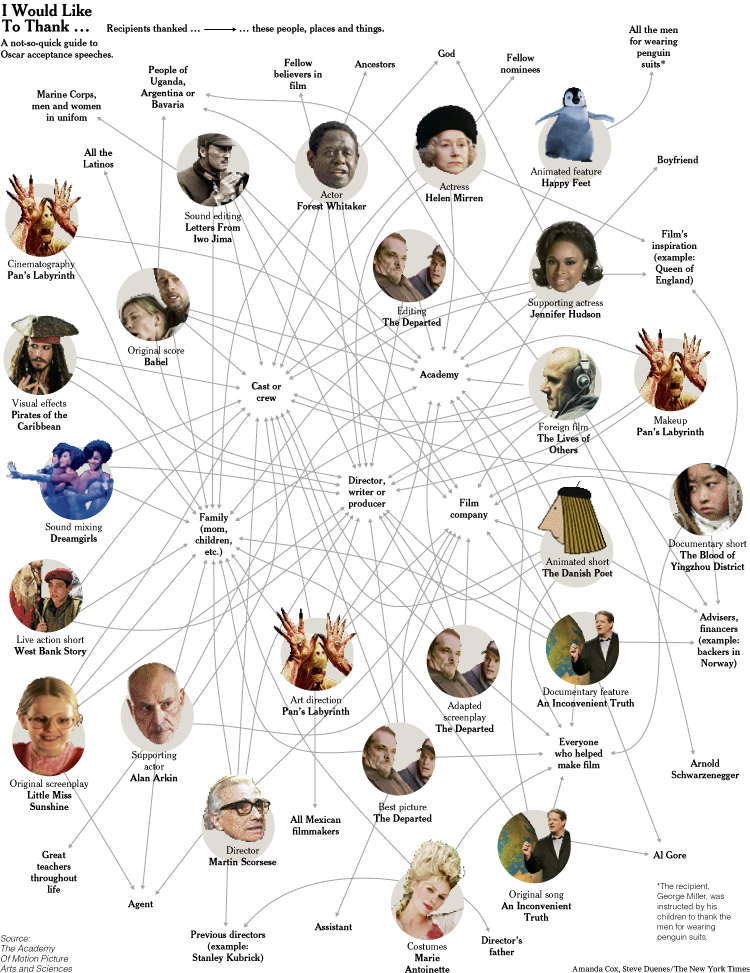
\includegraphics[height=0.9\textheight]{figures/nytimes_oscar_2007}
\end{center}

\vf
\Tiny{\url{http://www.nytimes.com/imagepages/2007/02/26/movies/27graphic.ready.html}}

\end{frame}
%%%%%%%%%%%%%%%%%%%%%%%%%%%
\begin{frame}

\begin{center}
\includegraphics<1>[width=0.9\textwidth]{figures/trump_network}
\end{center}

\vf
\Tiny{\url{http://www.kimalbrecht.com/project/trump-connections/}}

\end{frame}
%%%%%%%%%%%%%%%%%%%%%%%%%%%
\begin{frame}

\begin{center}
\Large{Your turn}
\end{center}

\end{frame}
%%%%%%%%%%%%%%%%%%%%%%%%%%%
\begin{frame}

\begin{center}
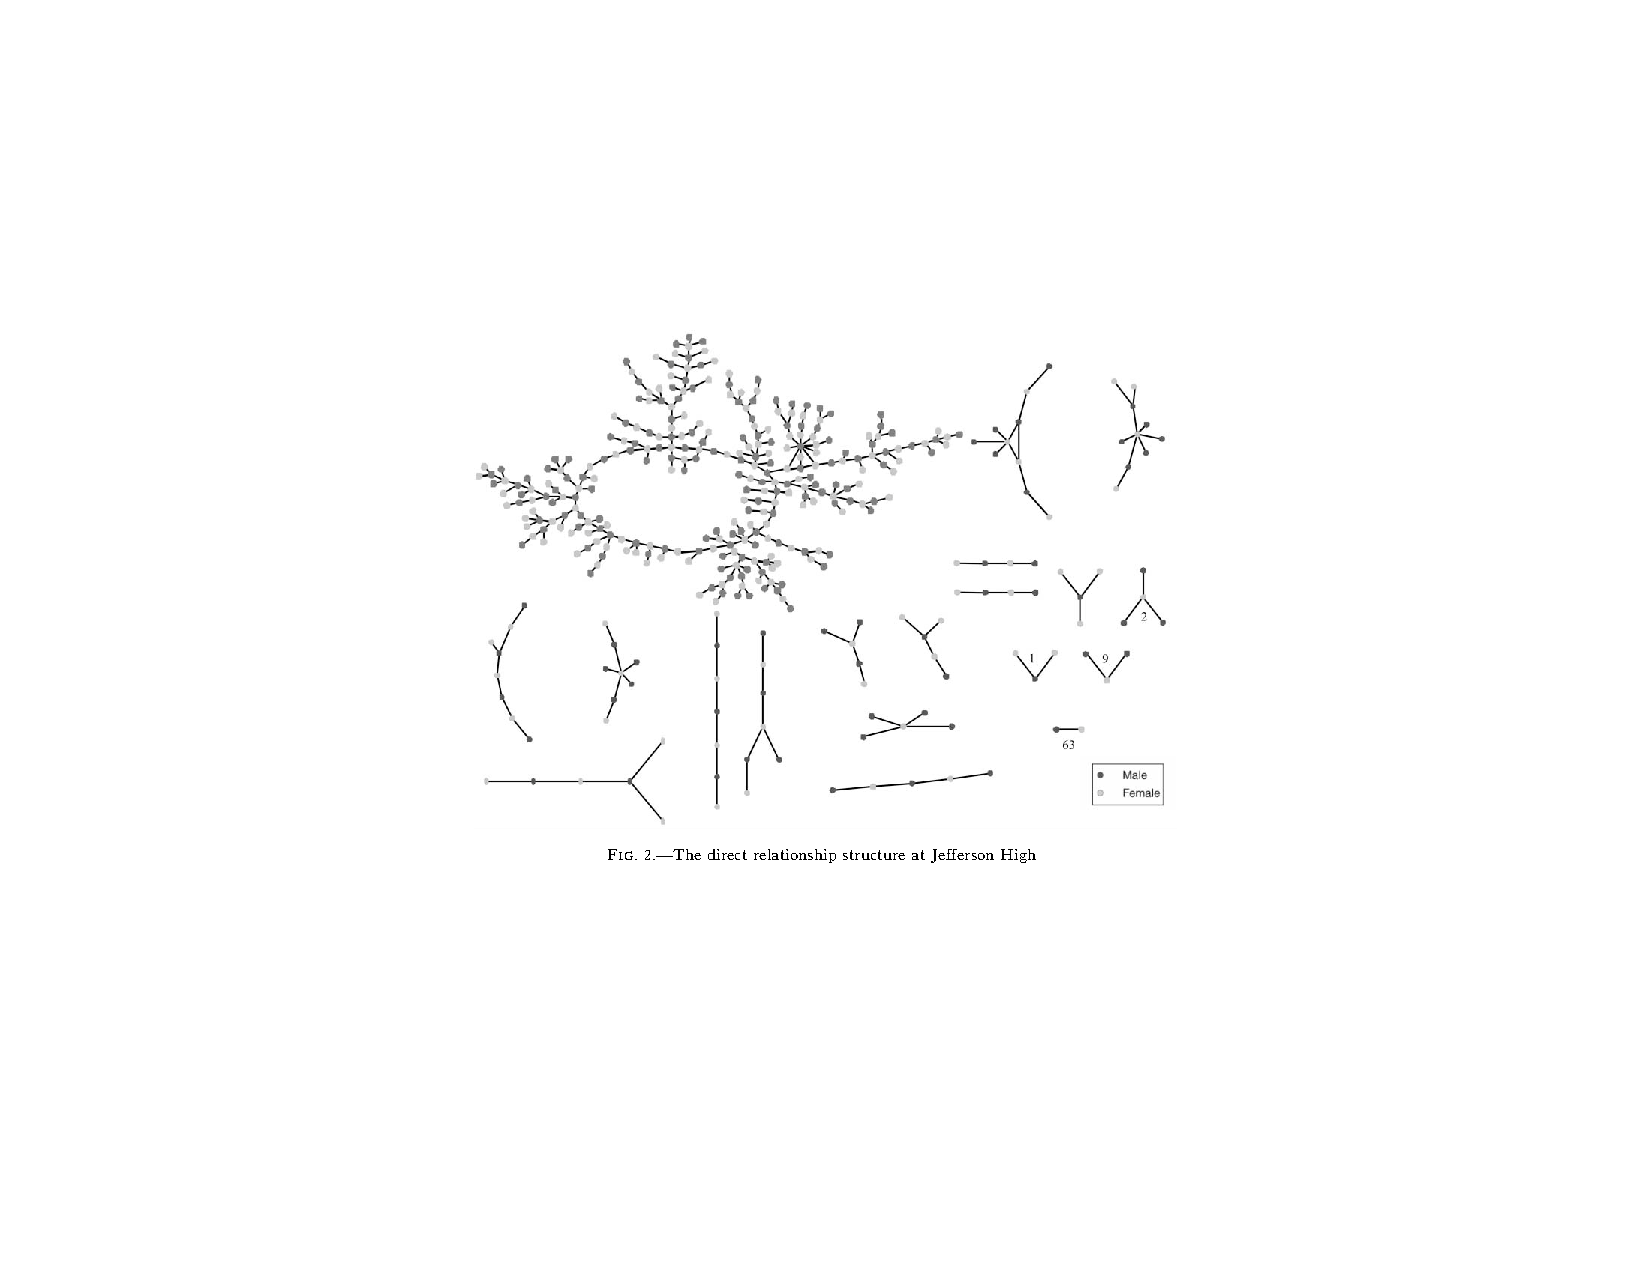
\includegraphics[width=0.95\textheight]{figures/bearman_chains_2004_fig2}
\end{center}

\vf
\Tiny{url{http://www.journals.uchicago.edu/doi/10.1086/386272}}

\end{frame}
%%%%%%%%%%%%%%%%%%%%%%%%%%%
\begin{frame}
\frametitle{}

\setcounter{subfigure}{0}
\begin{figure}
  \centering
     \subfigure[American High School]{
     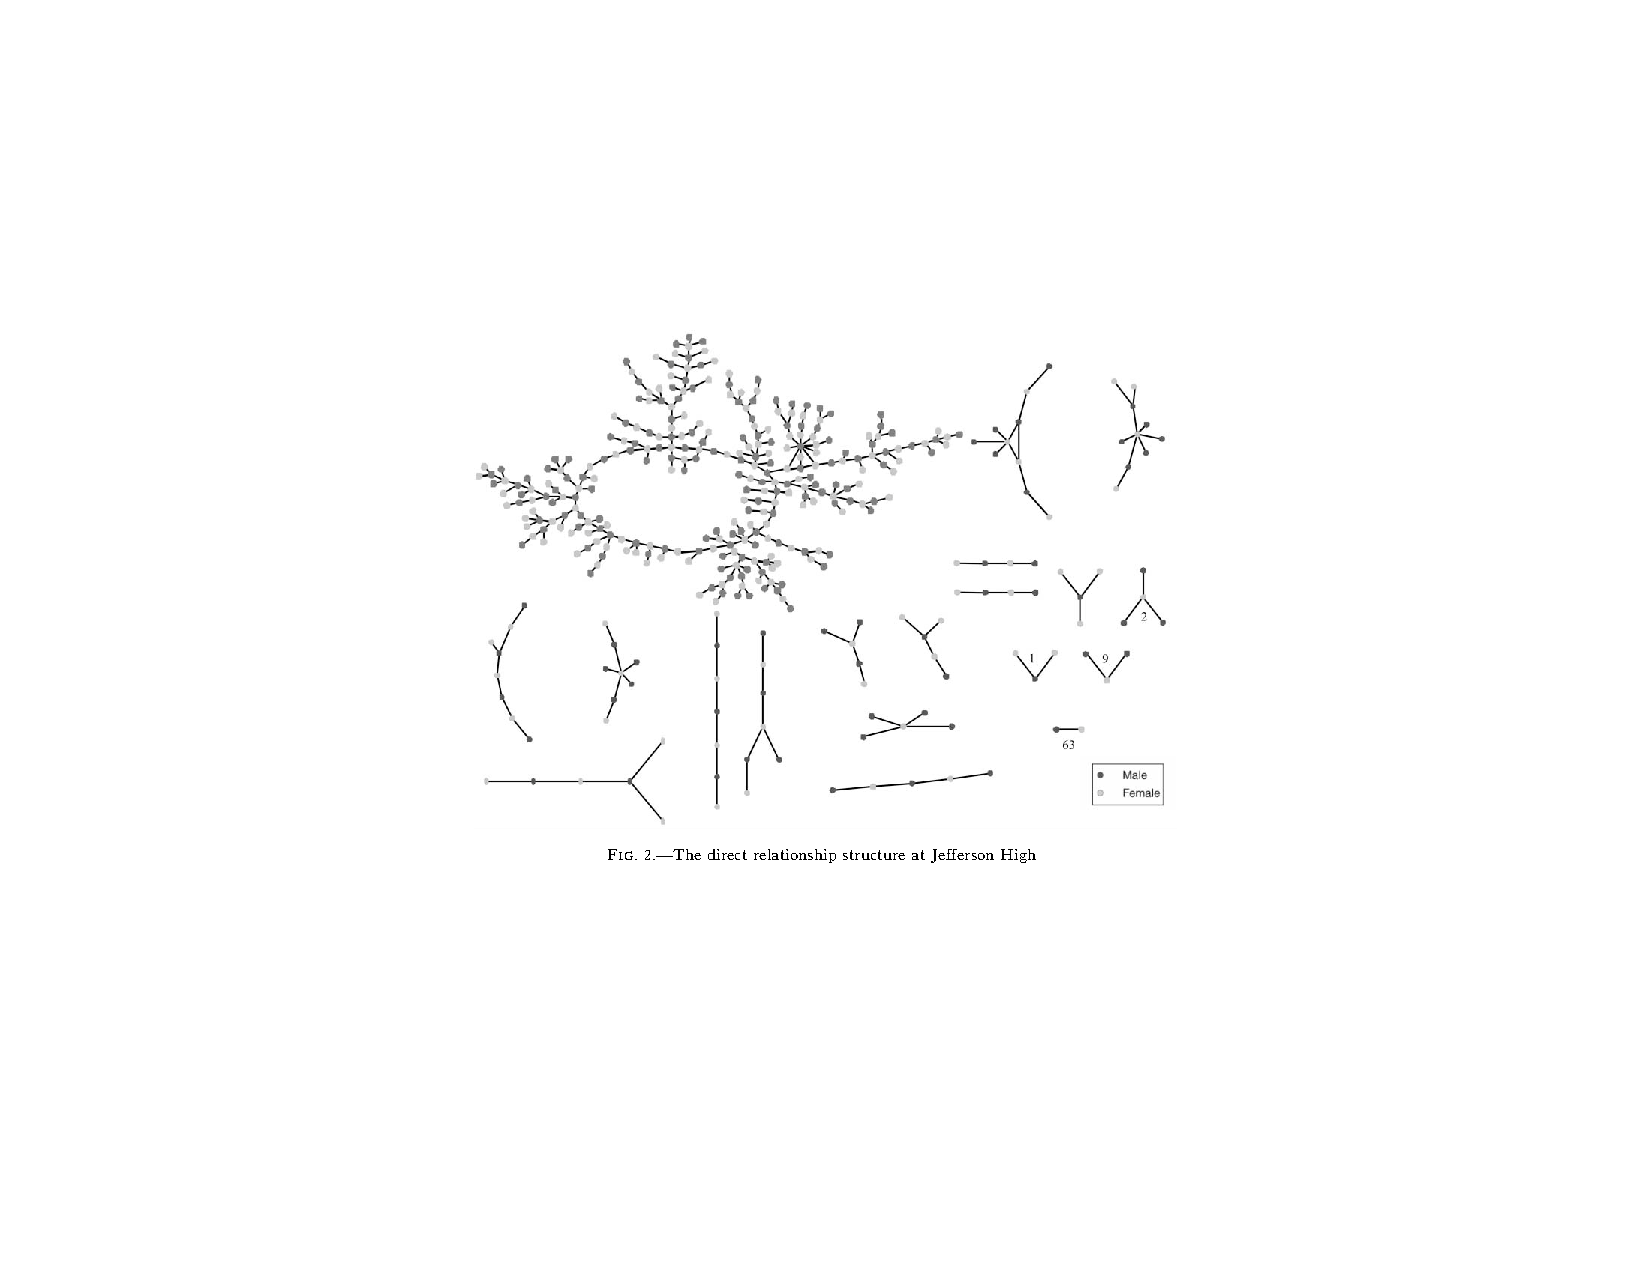
\includegraphics[width=0.45\textwidth]{figures/bearman_chains_2004_fig2}}
  \hspace{0in}
    \subfigure[Likoma Island, Malawi]{
    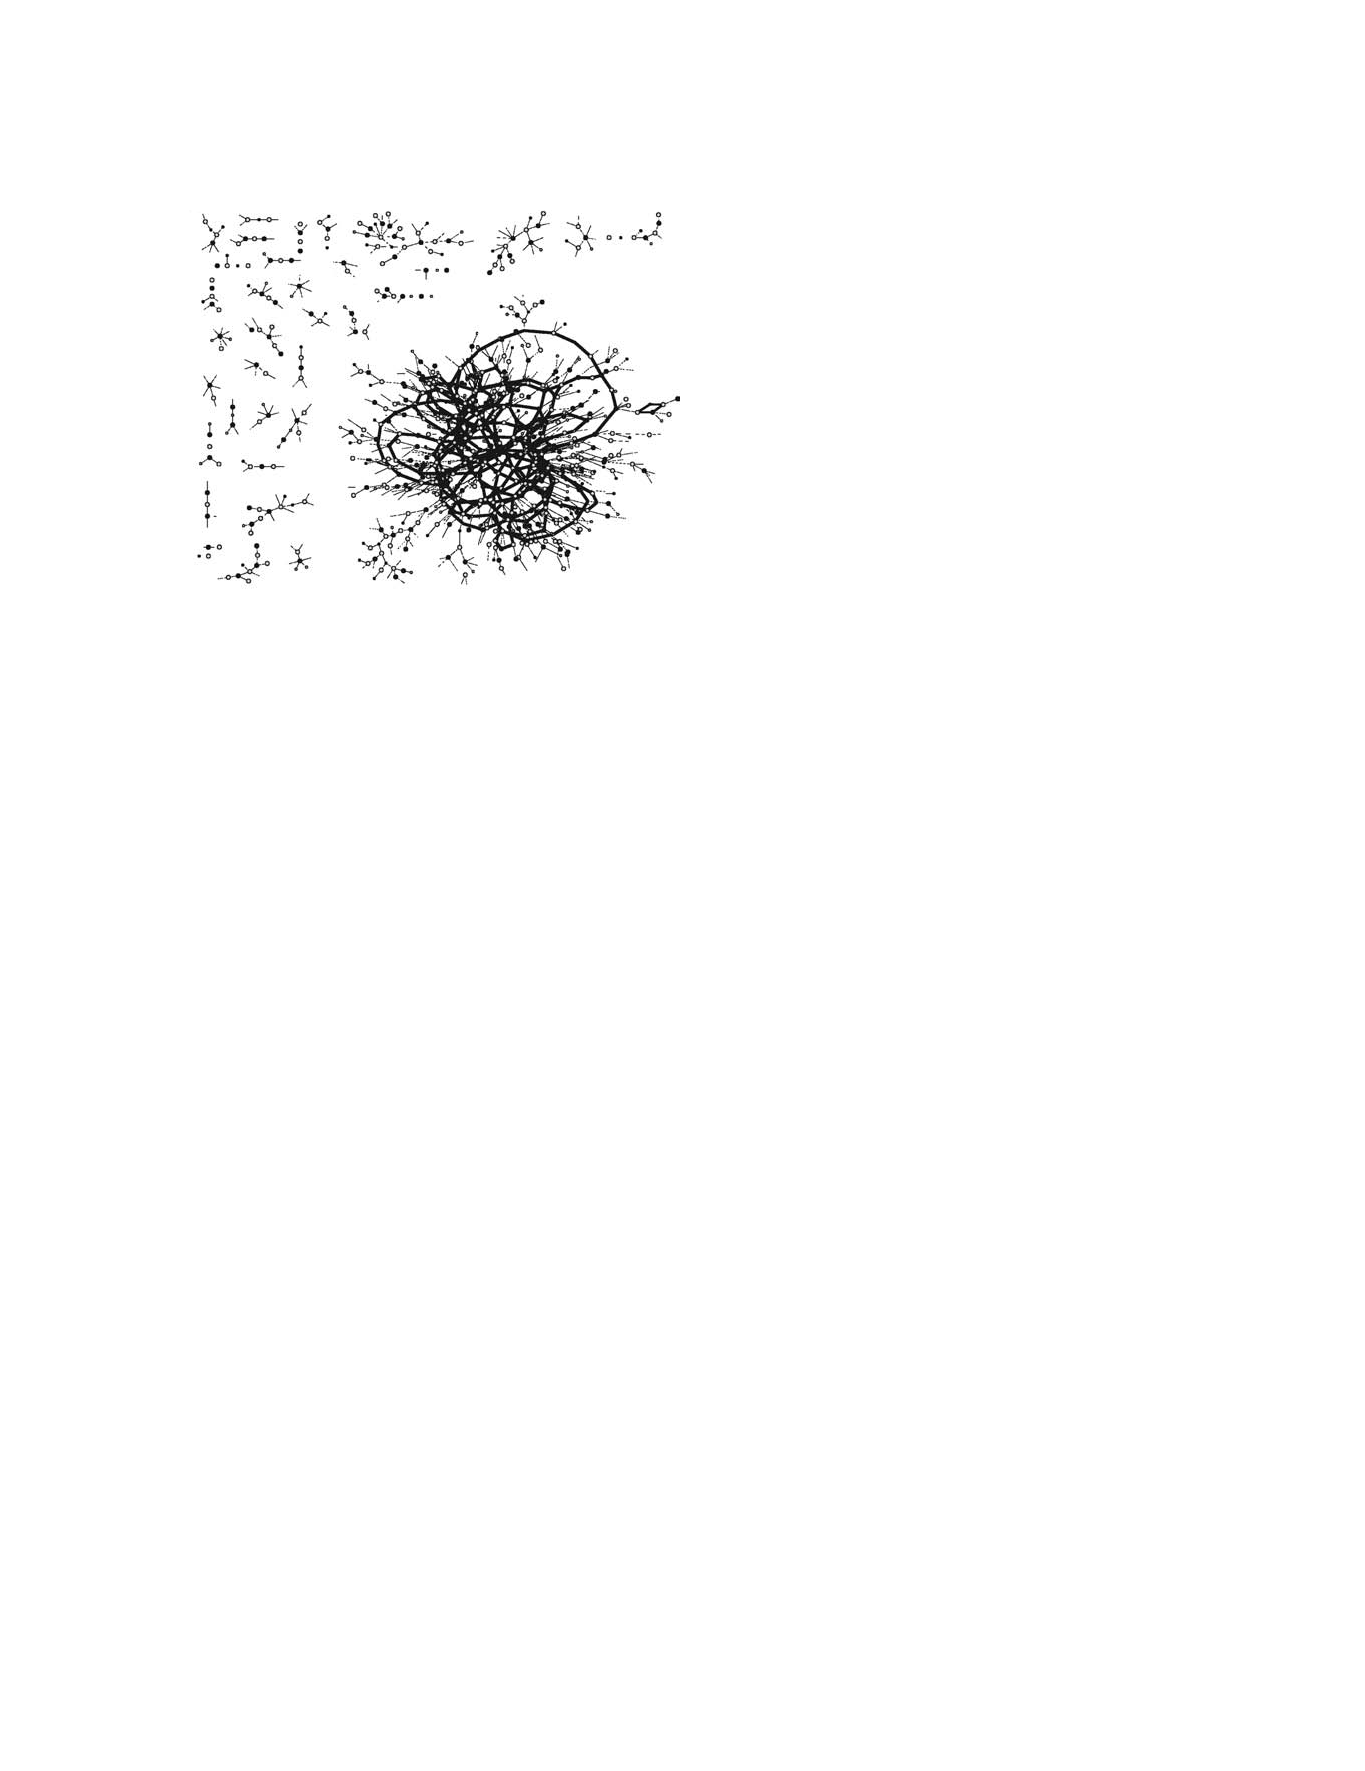
\includegraphics[width=0.45\textwidth]{figures/helleringer_sexual_2007_fig2a}}
\end{figure}

\vf
\Tiny{url{http://www.journals.uchicago.edu/doi/10.1086/386272} \& \url{https://www.ncbi.nlm.nih.gov/pubmed/18090281}}

\end{frame}
%%%%%%%%%%%%%%%%%%%%%%%%%%%
\begin{frame}

\begin{center}
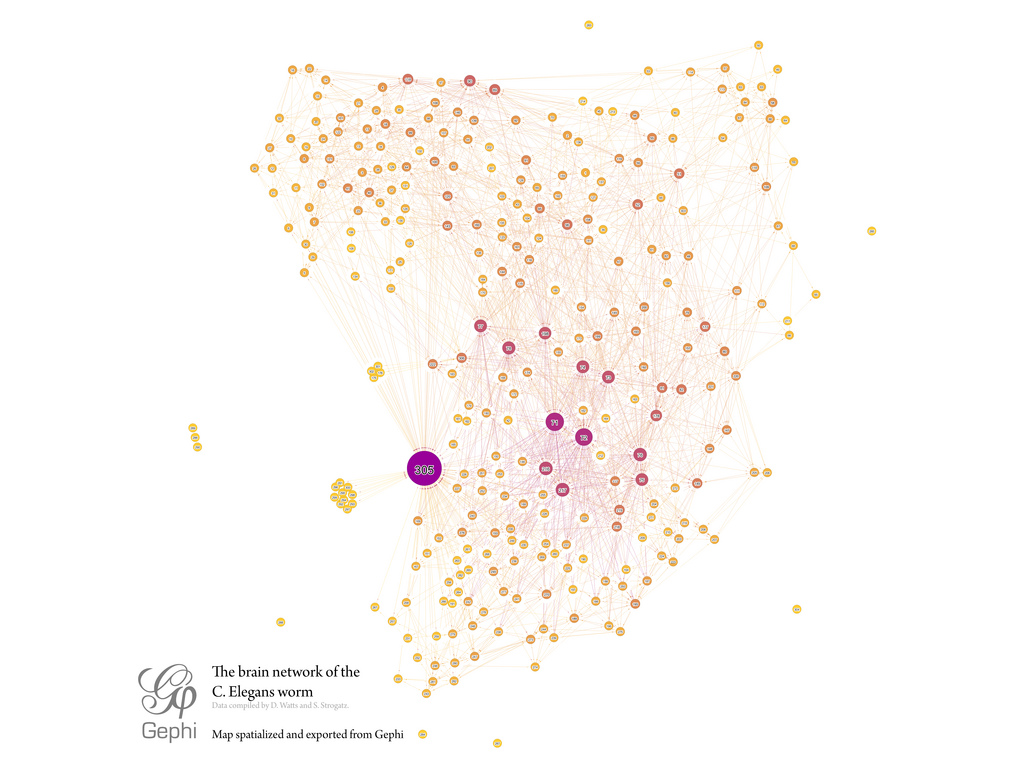
\includegraphics[width=0.95\textwidth]{figures/celegans_brain_network}
\end{center}

\vf
\Tiny{\url{https://commons.wikimedia.org/wiki/File:C.elegans-brain-network.jpg}}

\end{frame}
%%%%%%%%%%%%%%%%%%%%%%%%%%%
\begin{frame}

\begin{center}
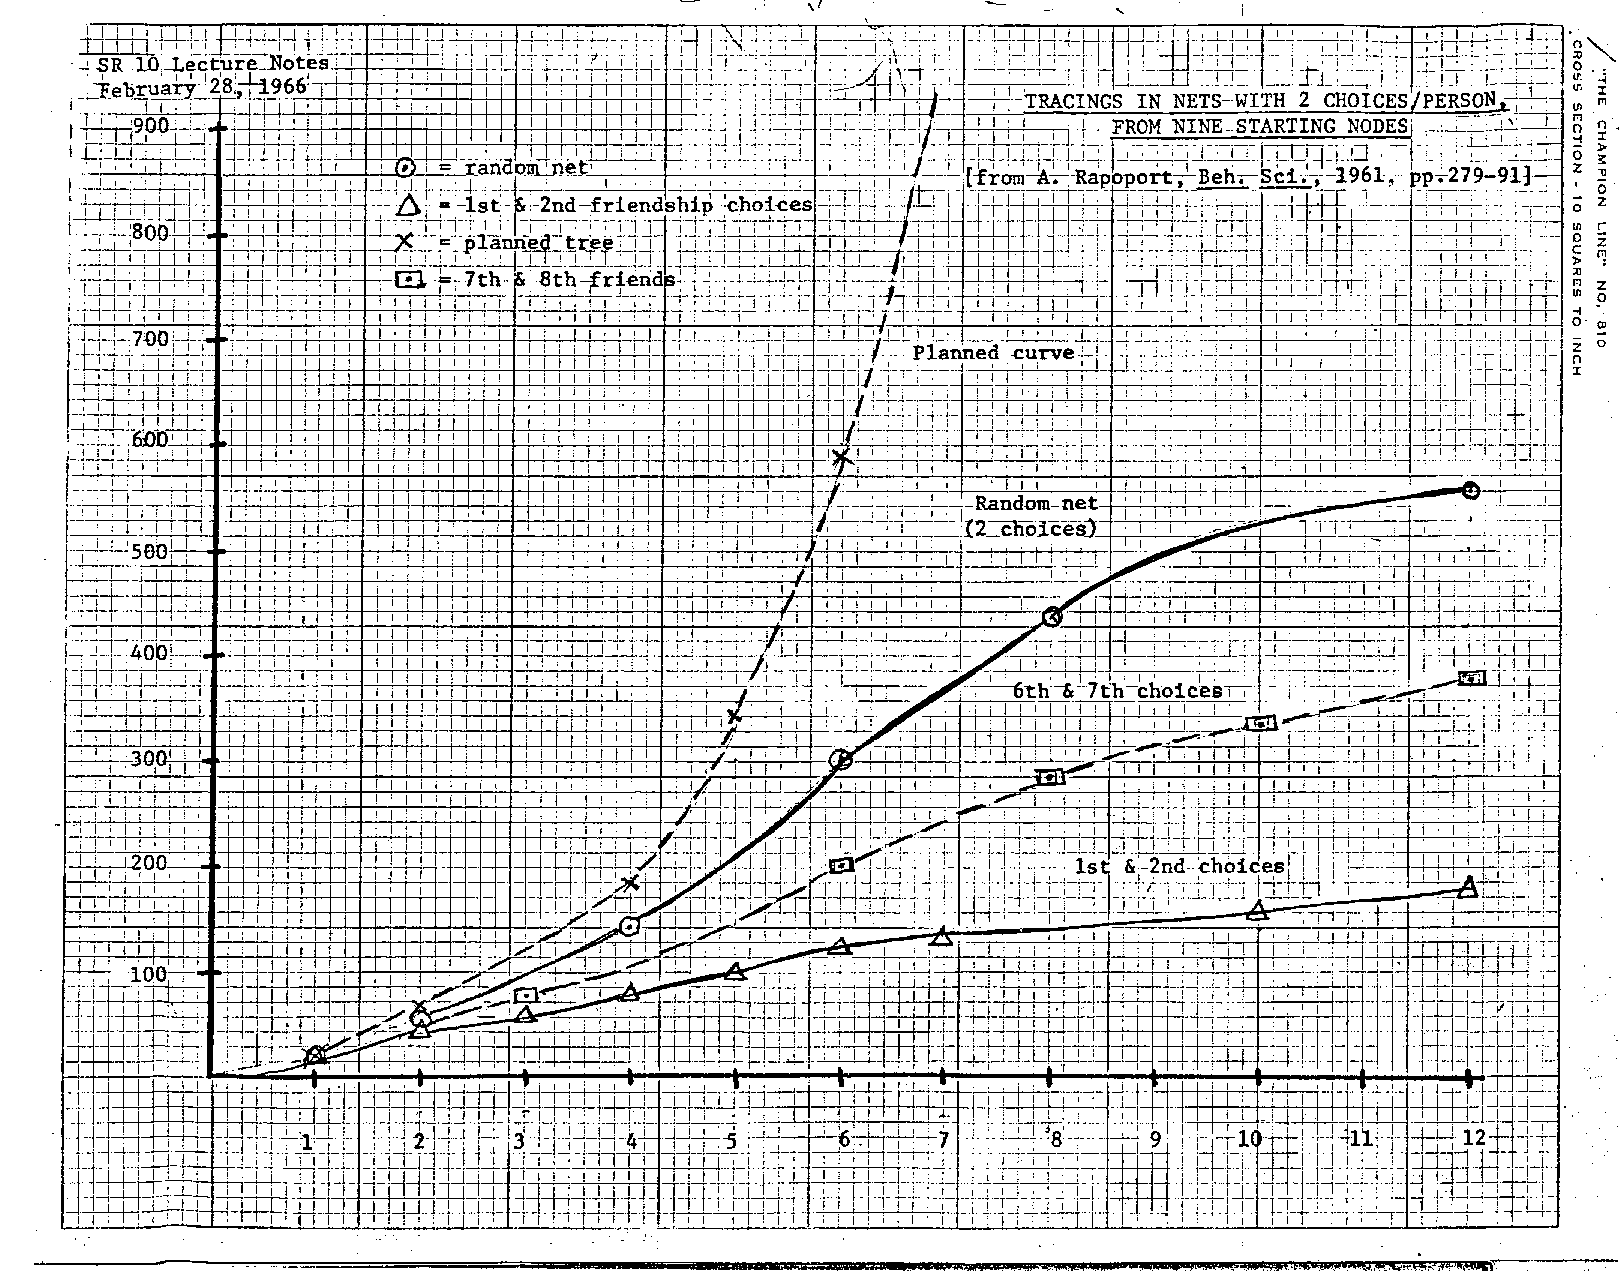
\includegraphics[width=0.95\textwidth]{figures/white_classnotes_swt}
\end{center}

\end{frame}
%%%%%%%%%%%%%%%%%%%%%%%%%%%
\begin{frame}

\begin{center}
\Large{Learning objectives}
\end{center}

\end{frame}
%%%%%%%%%%%%%%%%%%%%%%%%%%%
\begin{frame}

\begin{itemize}
\item Students will be able to \textbf{describe} the major concepts used in the study of networks.
\pause
\item Students will be able to \textbf{describe} the interconnections between the major concepts used in the study of networks.
\pause
\item Students will be able to \textbf{use} the major concepts in the study of networks to gain insight into real-world phenomena.
\pause
\item Students will be able to \textbf{evaluate} real, modern research that connects the concepts of networks to real-world phenomena.
\pause
\item Students will be able to \textbf{begin to create} new research that connects the major ideas and models of networks to real-world phenomena.
\end{itemize}

\end{frame}
%%%%%%%%%%%%%%%%%%%%%%%%%%%
\begin{frame}

\begin{center}
\Large{Major activities}
\end{center}

\end{frame}
%%%%%%%%%%%%%%%%%%%%%%%%%%%
\begin{frame}

\begin{center}
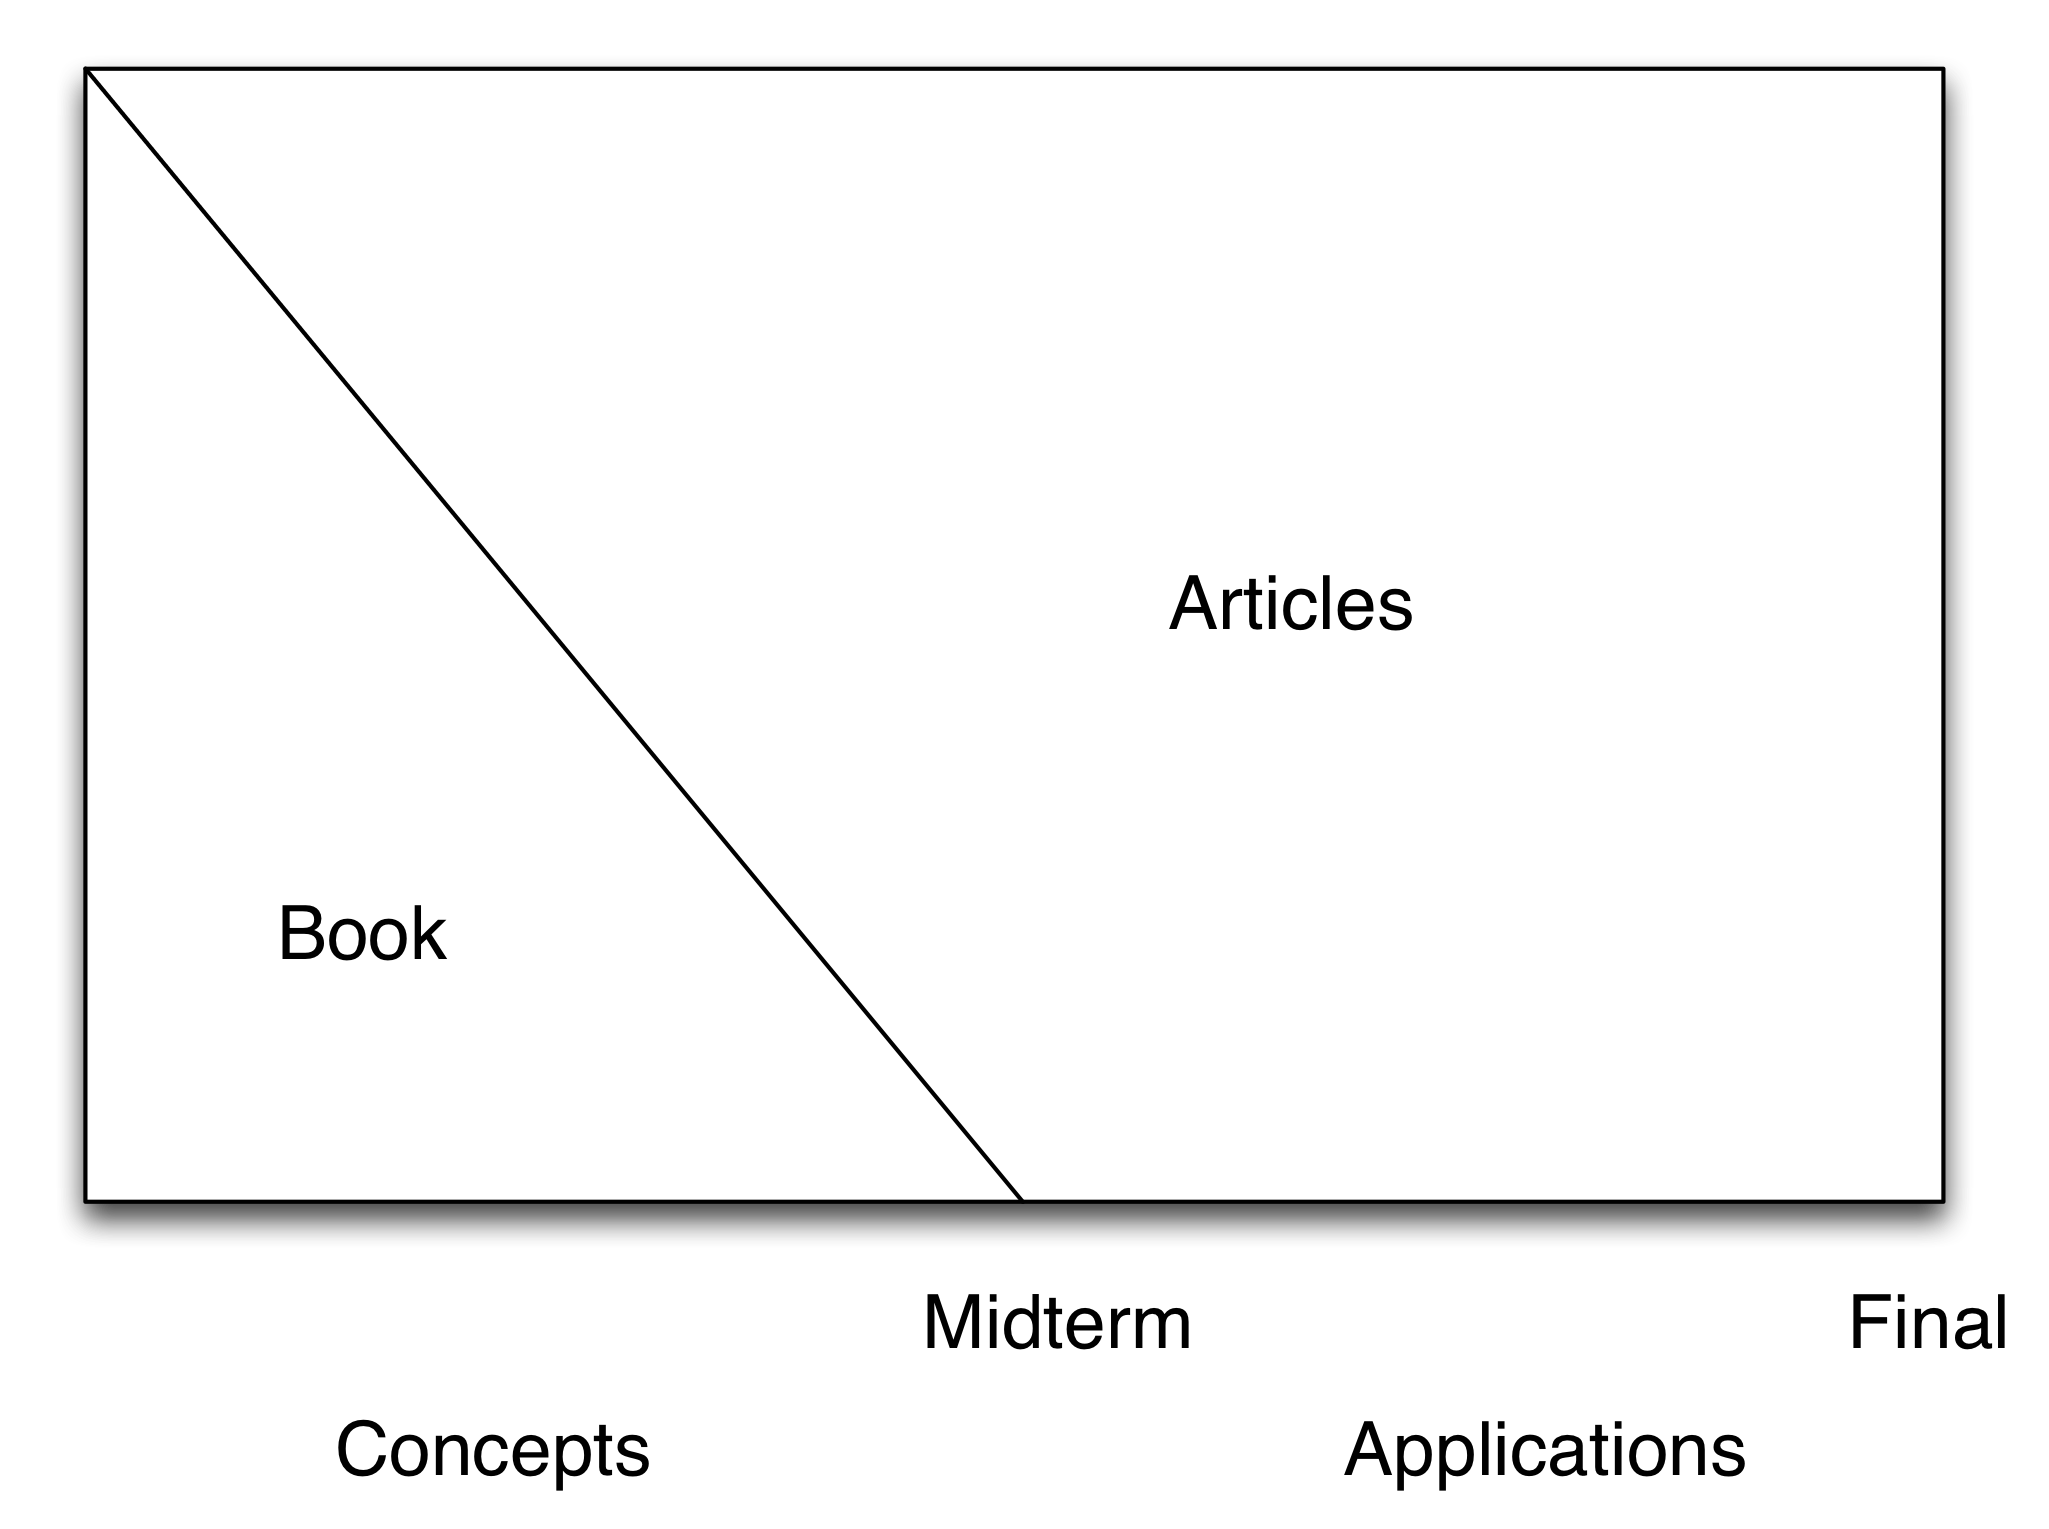
\includegraphics[width=0.95\textwidth]{figures/class_structure}
\end{center}

\end{frame}
%%%%%%%%%%%%%%%%%%%%%%%%%%%
\begin{frame}

\begin{itemize}
\item Midterm exam
\item Final exam
\item Weekly activities
\end{itemize}

\end{frame}
%%%%%%%%%%%%%%%%%%%%%%%%%%%
\begin{frame}

\begin{center}
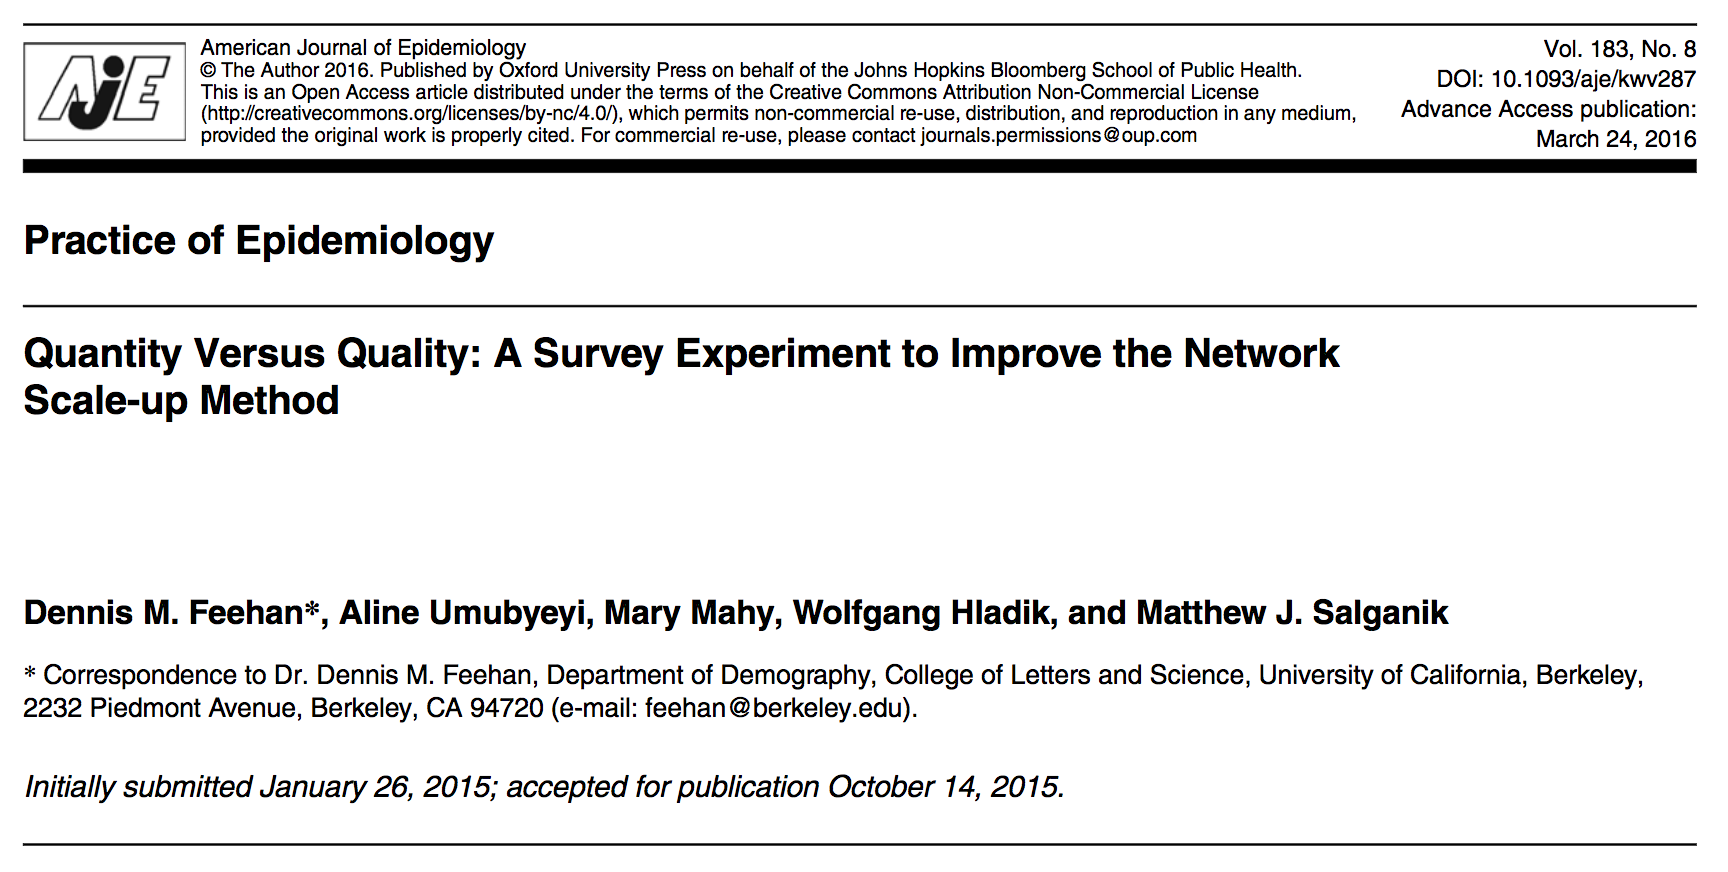
\includegraphics[width=0.95\textwidth]{figures/feehan_quality_2016_title}
\end{center}

\vf
\Tiny{\url{https://doi.org/10.1093/aje/kwv287}}

\end{frame}
%%%%%%%%%%%%%%%%%%%%%%%%%%%
\begin{frame}

\begin{center}

\includegraphics[width=0.95\textwidth]{figures/kramer_experimental_2014_title}
\end{center}

\vf
\Tiny{\url{https://doi.org/10.1073/pnas.1320040111}}

\end{frame}
%%%%%%%%%%%%%%%%%%%%%%%%%%%
\begin{frame}

\begin{center}
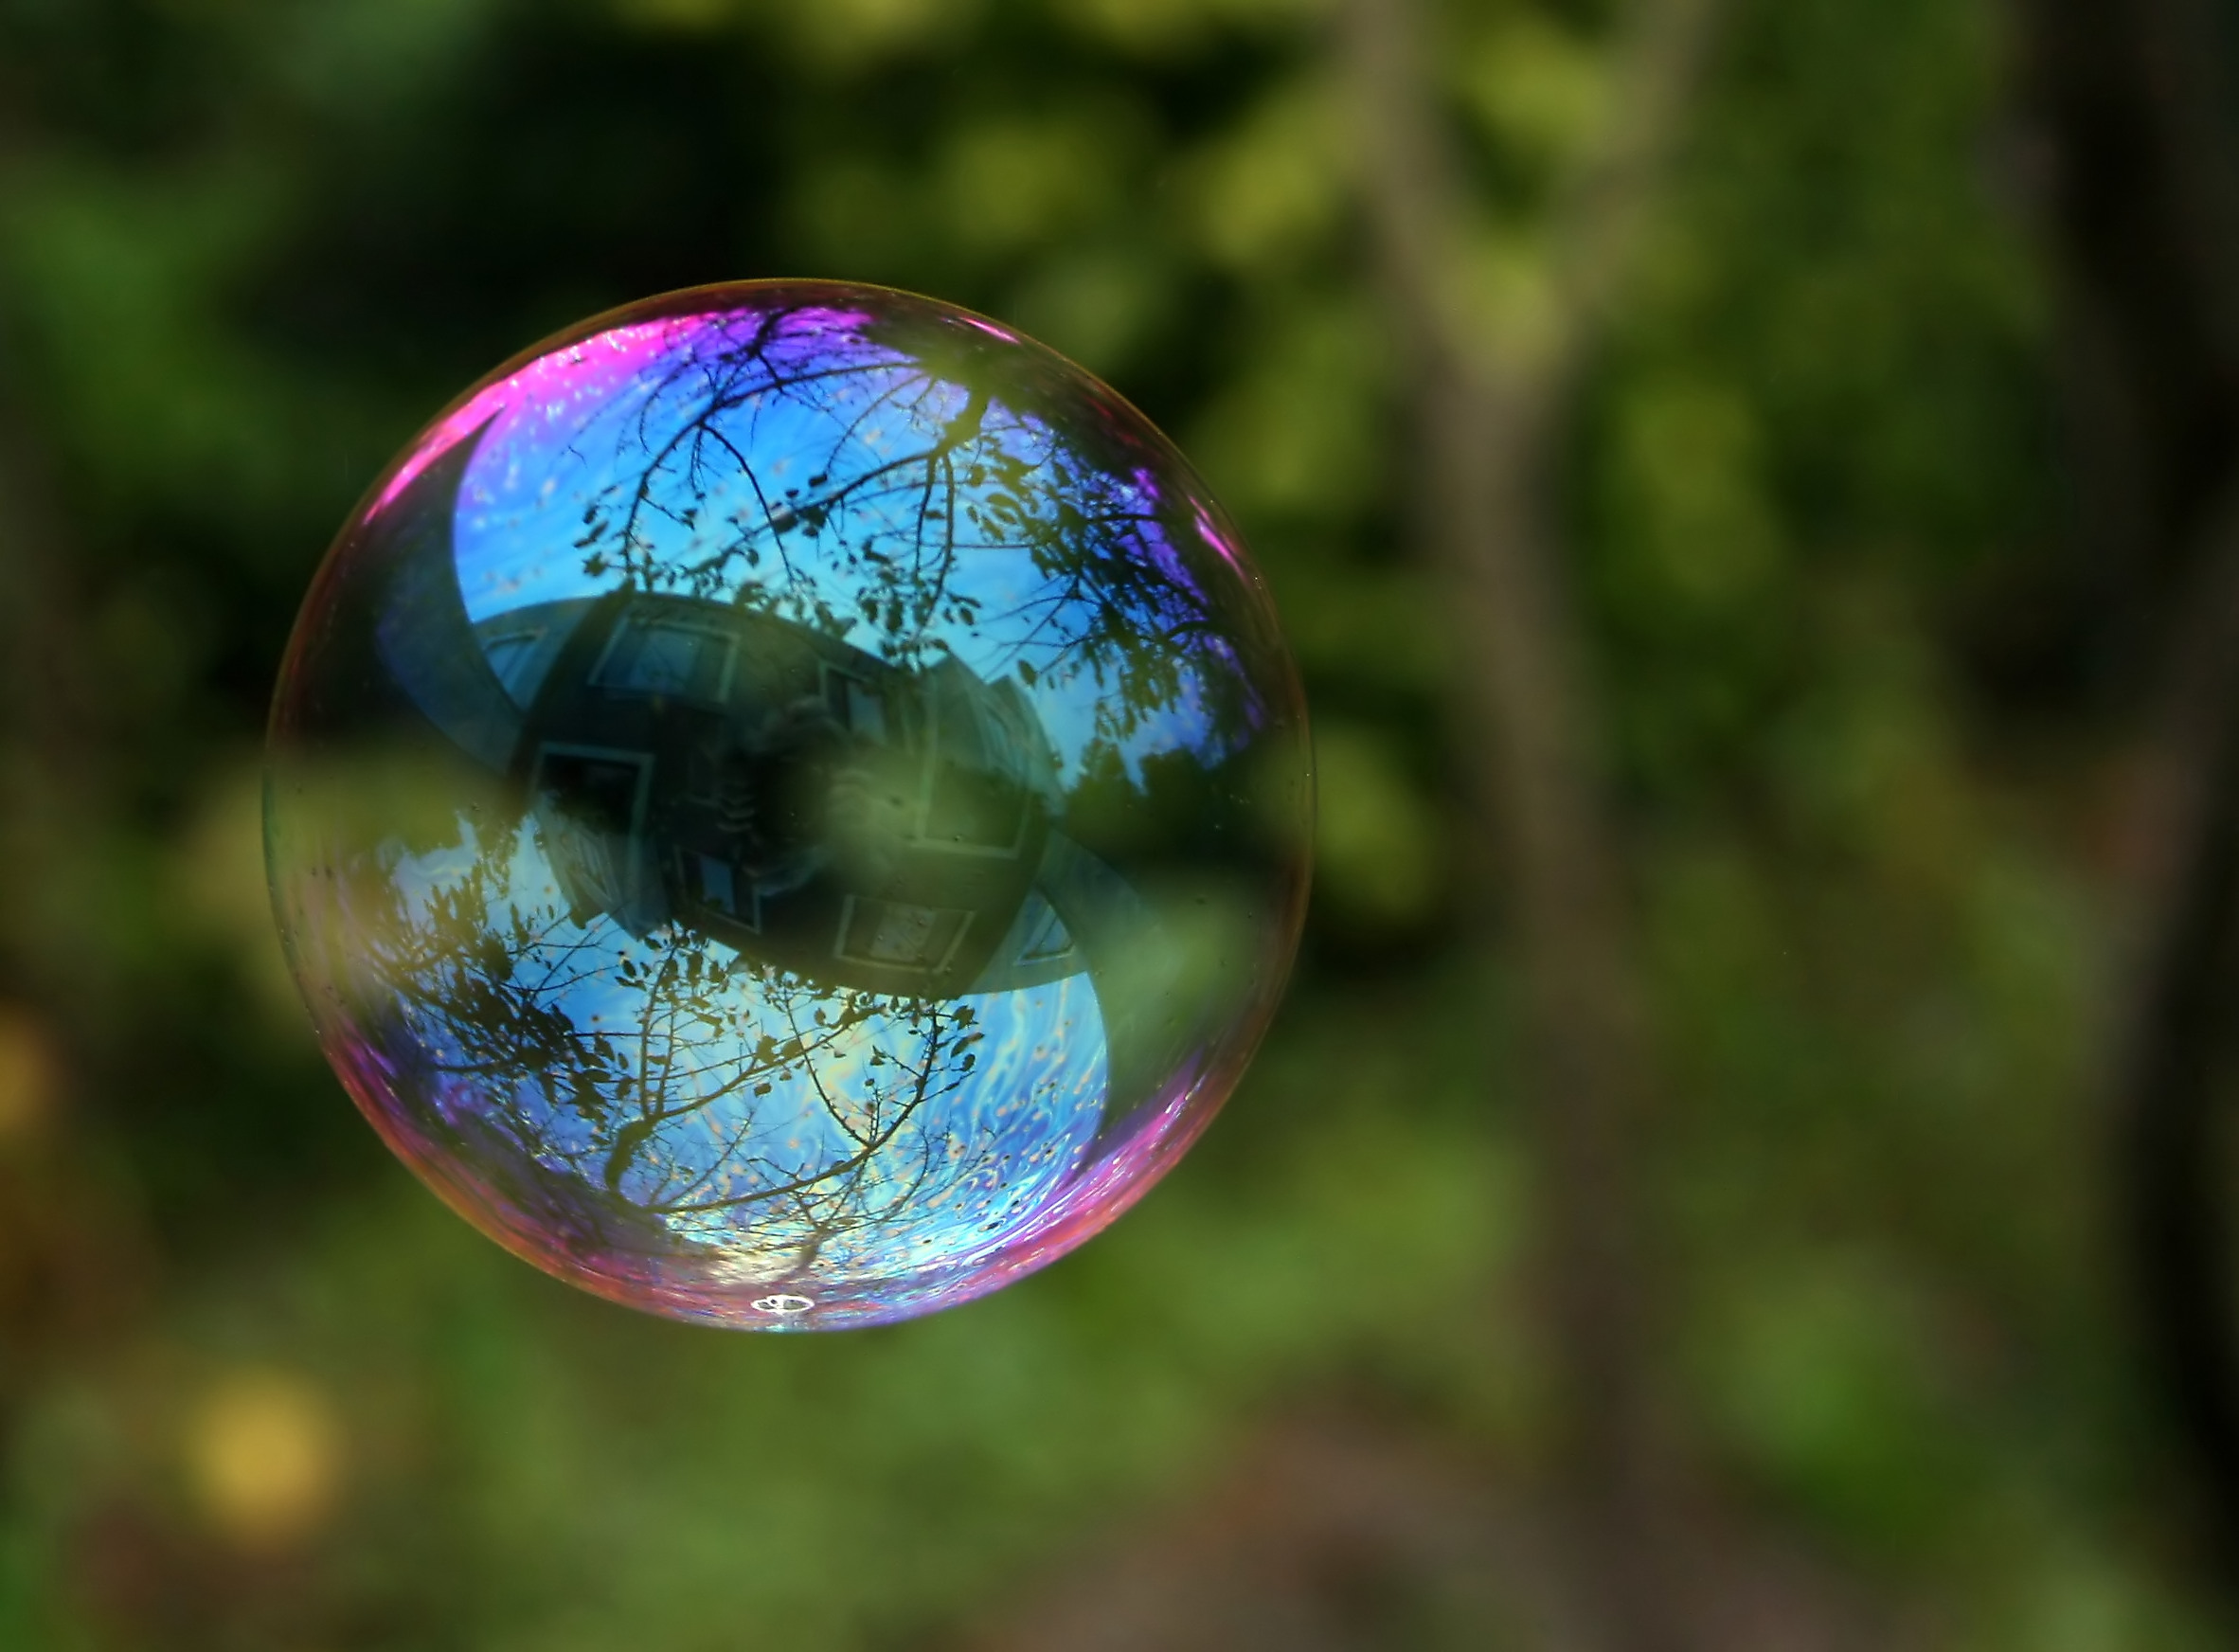
\includegraphics[width=0.95\textwidth]{figures/soap_bubble}
\end{center}

\vf
\Tiny{\url{https://commons.wikimedia.org/wiki/File:Reflection_in_a_soap_bubble_edit.jpg}}

\end{frame}
%%%%%%%%%%%%%%%%%%%%%%%%%%%
\begin{frame}

\begin{center}

\includegraphics[width=0.95\textwidth]{figures/princeton_precept}
\end{center}

\vf
\Tiny{\url{http://www.princeton.edu/pr/pub/precept/PU-Inspired-Conversations-2008.pdf}}

\end{frame}
%%%%%%%%%%%%%%%%%%%%%%%%%%%
\begin{frame}

\begin{center}
\Large{Getting to know each other}
\end{center}

\end{frame}
%%%%%%%%%%%%%%%%%%%%%%%%%%%
\begin{frame}

\begin{center}
\Large{About me}
\end{center}

\end{frame}
%%%%%%%%%%%%%%%%%%%%%%%%%%%
\begin{frame}

About the preceptors:
\pause
\begin{itemize}
\item Samuel Clovis
\item Romain Ferrali
\item Herrissa Lamothe
\item Sarah Reibstein
\item Janet Xu
\end{itemize}
\pause
\begin{itemize}
\item Ryan Parsons
\item Ramina Sotoudeh
\end{itemize}

\end{frame}
%%%%%%%%%%%%%%%%%%%%%%%%%%%
\begin{frame}

Logistical notes:
\begin{itemize}
\item Precept times have not been set
\item There is no precept this week
\end{itemize}

\end{frame}
%%%%%%%%%%%%%%%%%%%%%%%%%%%
\begin{frame}

\begin{center}
\Large{About you}
\end{center}

\end{frame}
%%%%%%%%%%%%%%%%%%%%%%%%%%%
\begin{frame}

\begin{itemize}
\item first year, second year, third year, fourth year
\pause
\item no major, sociology major, social science (but not sociology), humanities, natural sciences, cs/engineering
\end{itemize}

\end{frame}
%%%%%%%%%%%%%%%%%%%%%%%%%%%
\begin{frame}

\begin{center}
\includegraphics<1>[width=0.5\textwidth]{figures/fb_logo}
\includegraphics<2>[width=0.5\textwidth]{figures/instagram_logo}
\includegraphics<3>[width=0.5\textwidth]{figures/twitter_logo}
\includegraphics<4>[width=0.5\textwidth]{figures/yikyak_logo}
\includegraphics<5>[width=0.5\textwidth]{figures/questionmark}
\end{center}

active user (6 of past 7 days), have account, no account

\end{frame}
%%%%%%%%%%%%%%%%%%%%%%%%%%%
\begin{frame}

\begin{center}
\Large{Is this course right for you?}
\end{center}

\end{frame}
%%%%%%%%%%%%%%%%%%%%%%%%%%%
\begin{frame}

\begin{center}
\Large{Looking ahead}
\end{center}

\end{frame}
%%%%%%%%%%%%%%%%%%%%%%%%%%%
\begin{frame}

\begin{center}

\includegraphics[width=0.9\textwidth]{figures/haenschen_citp_facebook}
\end{center}

Facebook is the dominant social networking platform in the United States. This presentation offers a new method for conducting experiments within existing Facebook networks, without the express participation of Facebook itself. The theoretical rationale for this method is discussed, and four experiments are presented that use the method to explore the effects of social networks on political behaviors and attitudes. 

\vf
\Tiny{\url{http://citp.princeton.edu/event/haenschen/}}

\end{frame}
%%%%%%%%%%%%%%%%%%%%%%%%%%
\begin{frame}

\begin{itemize}
\item Watts, Preface and Chapter 1. (Available from Blackboard)
\item Milgram, S. (1967). The small world problem. \textit{Psychology Today}, 1:62-67. (Available from Blackboard)
\item Travers, J. and Milgram, S. (1969). An experimental study of the small world problem. \textit{Sociometry}, 32(4):425-443.
\item Kleinfeld, J.S. (2002). The small world problem. \textit{Society}, 39(2):61-66. (Available from Blackboard)
\end{itemize}

\pause
Arc: Background context $\rightarrow$ Informal Insight  $\rightarrow$ Formal Research $\rightarrow$ Critique \pause $\rightarrow$ Improved Research \\
\pause
While you are reading:
\begin{itemize}
\item think about the relationship between Watts' description and the actual studies
\pause
\item think about the connection between the informal insight and the formal research
\end{itemize}

\end{frame}
%%%%%%%%%%%%%%%%%%%%%%%%%%%





\end{document}
